\documentclass{article}

% Language setting
% Replace `english' with e.g. `spanish' to change the document language
\usepackage[english]{babel}

% Set page size and margins
% Replace `letterpaper' with `a4paper' for UK/EU standard size
\usepackage[letterpaper,top=2cm,bottom=2cm,left=3cm,right=3cm,marginparwidth=1.75cm]{geometry}

% Useful packages
\usepackage{amsmath}
\usepackage{amsfonts}
\usepackage{graphicx}
\usepackage{subcaption}
\usepackage{float}
\usepackage[colorlinks=true, allcolors=blue]{hyperref}

\title{Rapport Statistique  descriptive}
\author{MEDJKOUH Khaled \\ RAZAFINDRAKOTO Davidson Lova}

\begin{document}
\section{Introduction}

Understanding if a machine learning model is making accurate predictions or simply guessing at random is not trivial.

Bayesian machine learning seems to provide the solution, in the article, a new gradient-free training algorithm based on Approximate Bayesian Computation by Subset Simulation is proposed. In the proposed method, the likelihood function and the weights are defined by non-parametric formulations.

The experiments, especially the engineering case study on composite materials subject to fatigue damage, show the ability of the proposed algorithm to consistently reach accurate predictions while avoiding gradient related instabilities, and most importantly, it provides a realistic and coherent quantification of the uncertainty represented by confidence bounds which will be illustrated in the figures bellow.


\href{https://www.youtube.com/watch?v=p1EnIbDItTc}{Little video tutorial on How to handle Uncertainty in Deep Learning}

\section{Background}
\subsection{FNN (\href{https://en.wikipedia.org/wiki/Feedforward_neural_network}{Feedfoward Neural Network}) and BNN (Bayesian Neural Network)}

Let $D = (x,y) \in \mathcal{X} \times \mathcal{Y} \subseteq \mathbb{R}^m \times \mathbb{R}^l$ be the distribution of the dataset.

Let $\mathcal{M}$ be a model (here it is a FNN) with parameters $\theta = \{w ,b\}$ (où $w$ are the weights and $b$ the biais).

BNN consists of esmitimating the a posteriori distribition $p(\theta |D , \mathcal{M})$ of $\theta$ assuming the model $\mathcal{M}$ and the data set $D$ (whereas a stan<dard FNN just gives one point estimation of $\theta$). Here we have an FNN on the left and BNN on the right.

\begin{center}
    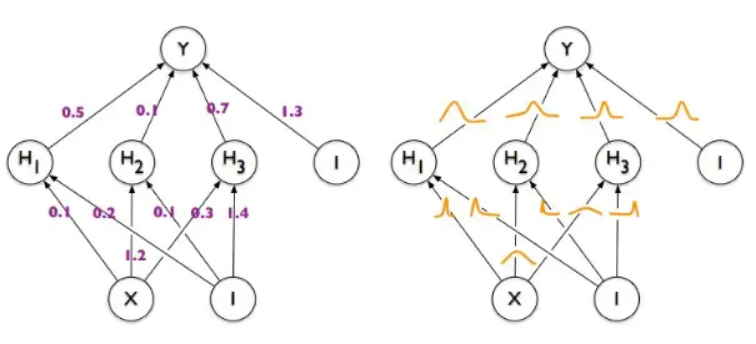
\includegraphics[width = 7cm]{./photo/BNN vs FNN.png}
\end{center}


\subsection{Approximate Bayesian computation by subset simulation}

\subsubsection{ABC (\href{https://en.wikipedia.org/wiki/Approximate_Bayesian_computation}{Approximate Bayesian Computation})}

    A feedforward pass of the FNN $\mathcal{M}$  with the input $x$ and $\theta \sim p(\theta, \mathcal{M})$ gives $\hat{y} = f(x, \theta)$ 

    The ABC algorithm consists at simulating samples of $\theta$, with theses samples, generating samples of $\hat{y}$ and keeping the $\theta$'s whose respective $\hat{y}$ are close to $y$. And with theses samples estimate $p(\theta | D, \mathcal{M})$.

\subsubsection{SS (\href{https://en.wikipedia.org/wiki/Subset_simulation}{Subset Simulation})}

    ABC is thus based on a rejection method, where we want the quantity $\rho(\eta(\hat{y}, \eta(y)))$ to get bellow a tolerance $\epsilon$ ($\rho$ is a dissimilarity measure and $\eta$ is a summarizing statistic).
    
    The subset simulation method is used to reach tolerance faster. It is a iterative method where we begin with a high tolerance, we generate samples using a portion the previous batch(which has $\hat{y}$s closest to $y$) and shrinking the tolerance. We iterate until we get a tolerance smaller than $\epsilon$.

    Since each time we use the best samples to generate the next batch in the next iteration, we go faster.

\section{Training BNN By ABC-SubSim}
\subsection{Proposed Methodology}

First choose a sample size $N$, $p_0 \in [0,1]$ such that $p_0\times N$ and $p_0^{-1} \in \mathbb{Z}^*$

1.  Generate $N$ samples of $\theta = \{w,b\}$ from it's prior user defined PDF $p(\theta|\mathcal{M})$

2.  Use them to run a forward pass and obtain $N$ outputs $\hat{y}(\theta)$.

3.  Evaluate the metric $\rho(\eta(\hat{y}), \eta(y))$ for each sample ${\theta, \hat{y}(\theta)}$.

4.  Keep $p_0\times N$ $\theta$ with the lowest metric value $\rho$ as seeds.

5.  These seeds are used to:

\begin{itemize}
    \item automatically fix the tolerance value $\epsilon_j$, as the highest metric value $\rho$ among the seeds.
    \item obtain $p_0^{-1}$ new samples from each seed verifying $\rho \leq \epsilon_j$ using the Modified
Metropolis Algorithm (MMA).
\end{itemize}

6. repeat the process until $\epsilon_j \leq \epsilon$

 The distribution of parameters in the final subset constitute the marginalized posterior $p_{\epsilon}( \theta | D, \mathcal{M})$ whose information is used to produce robust predictions and quantify their uncertainty.

\subsection{Illustrative Problems }

The aim is to do estimate from noised data. 
$y = cos(x) + \zeta$ where $\zeta \sim \mathcal{N}(0.1)$

    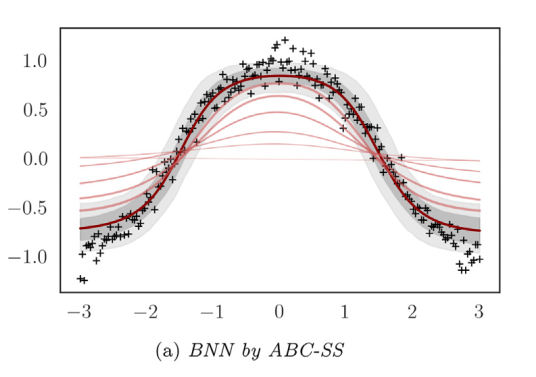
\includegraphics[width=5cm]{./photo/fig3_a.png}
  \hfill
    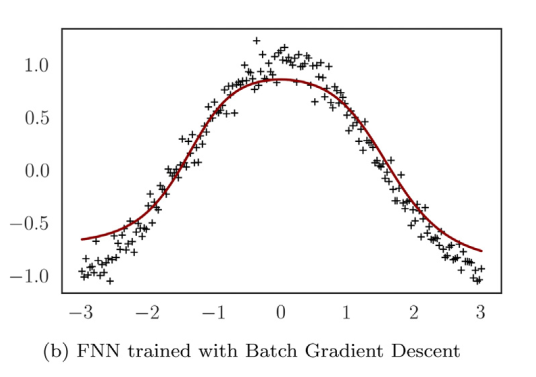
\includegraphics[width=5cm]{./photo/fig3_b.png}

$y = 10 sin(2 \pi x) + \zeta$ where $\zeta \sim \mathcal{N}(0.1)$
    
    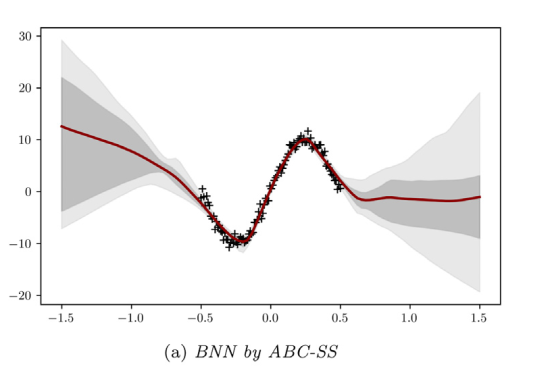
\includegraphics[width=5cm]{./photo/fig5_a.png}
    \hfill
    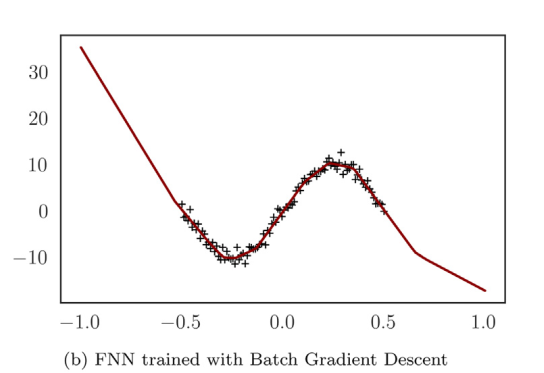
\includegraphics[width=5cm]{./photo/fig5_b.png}
    
\subsection{ Case Study}

    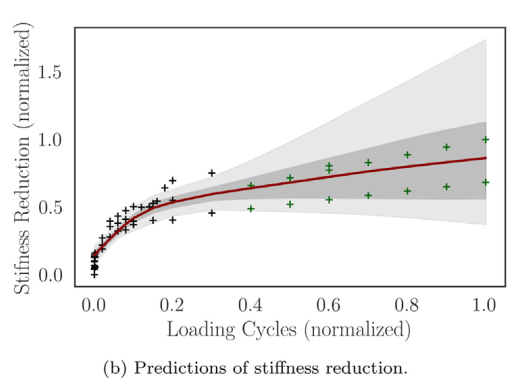
\includegraphics[width=5cm]{./photo/fig8_a.png}
    \hfill
    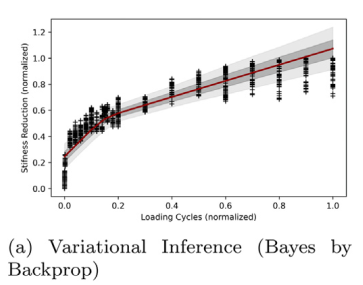
\includegraphics[width=5cm]{./photo/fig10_a.png}

    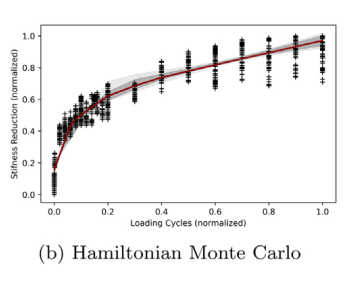
\includegraphics[width=5cm]{./photo/fig10_b.png}
    \hfill
    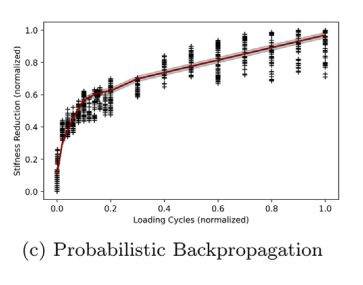
\includegraphics[width=5cm]{./photo/fig10_c.png}

\end{document}